\section{Pla d'acció}
\subsection{Diagrama de Gantt}
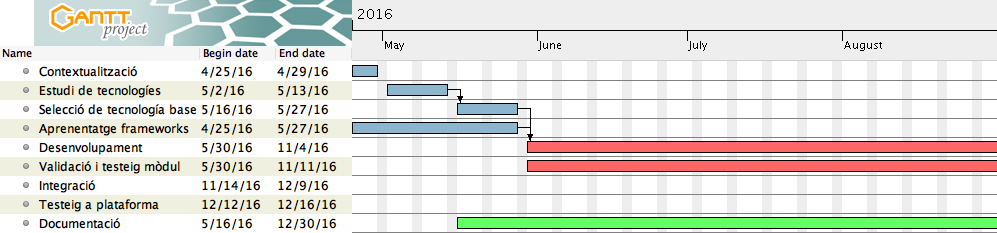
\includegraphics[scale=0.5]{img/ganttHPart1.png}	
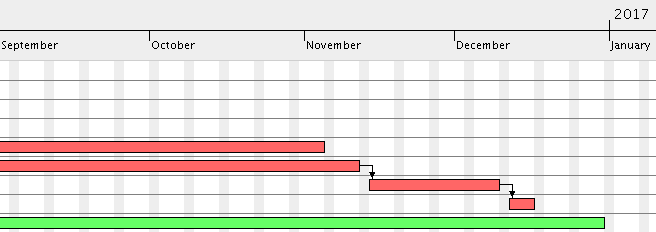
\includegraphics[scale=0.5]{img/ganttHPart2.png}	

\subsection{Interpretació}
Com es pot apreciar al diagrama anterior, la planificació està prevista per a que el projecte, començant juntament amb el conveni el 25 d'abril d'aquest mateix any, finalitzi en acabar l'any.\\
\newline Dins del projecte, tal i com es pot haver apreciat durant l'explicació de les tasques, podem trobar tres fases clarament diferenciades.
\renewcommand{\labelenumi}{\roman{enumi}}
\begin{enumerate}
	\item En aquesta primera part, marcada en el diagrama de gantt anterior amb color blau, es pretén asentar les bases per al posterior desenvolupament, adquirir tots, o si més no gran part,  els coneixements necesaris per a dur a bon port el futur desenvolupament.\\
		\newline En aquesta primera fase s'hi inclou, la lectura i anàlisi de les diferents lleis sobre signatura, investigació sobre possibles tencologíes i camins a seguir, així com agafar una mica de rodatge amb les tecnologíes emprades dins de la pròpia empresa.
	\item Seguidament, marcada a la figura anterior e color vermell, el gruix del projecte. Tot el desenvolupament on s'han d'aplicar tots els coneixements adquirits durant el transcurs de la fase anterior.\\
		\newline Aquesta fase inclou tot el procés de desenvolupament i testeig del mòdul, així com la seva posterior integració a la plataforma i el seu corresponent testeig.
	\item Finalment, es pot apreciar de color verd a la figura anterior, una fase que comença a mitjans de la fase de cerca: el procés de documentació.\\
		\newline És important que es documenti a mesura que es desenvolupa per tal del mantenir la informació al día, i que en un futur, la informació enmagatzemada dins d'aquesta documentació no sigui fruit del record del moment sobre una decisió concreta.
\end{enumerate}

